\documentclass[journal]{IEEEtran}
\usepackage[paper=letterpaper, textwidth=18.59cm, textheight=25cm, includehead]{geometry}
\usepackage[style=ieee]{biblatex}
\addbibresource{references.bib}
\ifCLASSINFOpdf
  \usepackage[pdftex]{graphicx}
\else
  \usepackage[dvips]{graphicx}
\fi
\usepackage{amsmath,amsthm,amsfonts,amssymb,amsxtra,mathtools,xfrac,nicefrac,siunitx,stmaryrd,cancel,relsize,steinmetz,braket,nicematrix}
\usepackage[math-style=ISO]{unicode-math}
\usepackage{etoolbox, array, float, subcaption, subfloat}
\usepackage{xcolor-material}
\usepackage{tikz, circuitikz}
\usetikzlibrary{arrows.meta, positioning}
\usepackage[luatex,hidelinks,%
			      pdfauthor={Antonios KAPETANIOS, Panagiotis PAPADOPOULOS},%
			      pdftitle={116 Design of VLSI Systems},%
			      pdfsubject={FinFET \& FD-SOI Technologies},%
			      pdfkeywords={FinFET, FD-SOI, VLSI}]{hyperref}
\makeatletter
\patchcmd{\@makecaption}
  {\scshape}
  {}
  {}
  {}
\makeatother

\newcommand{\RE}{\mathop{\symfrak{Re}}\nolimits}
\newcommand{\IM}{\mathop{\symfrak{Im}}\nolimits}

\DeclareSIUnit{\decade}{\symup{dec}}

% \usepackage{pgfplots}
% \pgfplotsset{compat=1.17}

\begin{document}
\markboth{[116]~Design~of~VLSI~Systems,~January~2026}{Group 02}

\title{[116] Design of VLSI Systems: Literature Report on FinFET and FD-SOI Technologies}
\author{
	\vfill{Group~02:~Antonios~KAPETANIOS~[10417],~\and~Panagiotis~PAPADOPOULOS~[10697]}\vfill
	\begin{center}
		{Aristotle University of Thessaloniki --- Faculty of Engineering\\
		Department of Electrical and Computer Engineering}
	\end{center}
}

	\NiceMatrixOptions{cell-space-limits = 2pt}
	\renewcommand{\arraystretch}{1.2}

	\maketitle

	\renewcommand{\arraystretch}{1.75}

	\begin{abstract}
		The purpose of this report is to briefly present and discuss FinFET and FD-SOI (Fully Depleted-Silicon On Insulator) devices. Four articles --published within the last two years-- were chosen to be discussed; \cite{FinFET1} and \cite{FinFET2} focus on FinFET devices, whereas \cite{FDSOI1} and \cite{FDSOI2} focus on devices in FD-SOI 22nm technology.
	\end{abstract}

	\section{Introduction}
		\IEEEPARstart{T}{he} continuous scaling of planar MOSFET structure on bulk silicon has been crucial to the evolution of VLSI \cite{Fossum_Trivedi_2013}. However, scaling has proven the long-channel transistor model to be insufficient \cite{Brennan_2005} as short-channel effects (SCEs) dominate \cite{Fossum_Trivedi_2013}\cite{Brennan_2005}. According to \cite{Fossum_Trivedi_2013} the most prominent candidates offering sufficient control over SCEs are FinFET and FD-SOI devices.\par

		Short channel effects (SCEs) are the effects, caused by scaling, that affect the device's behavior and intrinsic properties \cite{Brennan_2005}. Such effects are \textsl{charge sharing},  \textsl{drain-induced barrier lowering (DIBL)}, \textsl{carrier-velocity saturation}, and \textsl{hot carrier injection into the oxide} \cite{Brennan_2005} among others. These effects are explained below.\par

		The articles chosen to be discussed in this report mainly focus on the drain-voltage's influence on threshold voltage, $V_{\symup{th}}$, \cite{MOSFETArora}. \textbf{Drain-induced barrier lowering} (DIBL) occurs when the depletion layer formed around the drain begins to interact with the source-channel junction \cite{YangMicroelectronics}. Specifically, the surface potential near the source is lowered \cite{MOSFETArora} allowing electrons to be injected into the channel regardless of the voltage applied to the gate \cite{YangMicroelectronics}.

		When in the subthreshold region --that is $\left| V_{g} \right| \lneqq \left| V_{\symup{th}} \right|$-- and voltage is applied to the drain, then the drain current starts increasing \cite{FDSOICMOS}. When $V_{g}=0\unit{\volt}$ the drain current is not zero \cite{FDSOICMOS}\cite{KURINEC20015461}\cite{AGARWAL202381}\cite{FjeldlyVthModeling}. This non-zero drain current when the device should be ``off'' ($V_{g}=0\unit{\volt}$) is called \textsl{leakage current} and in VLSI it can increase significantly power dissipation \cite{KURINEC20015461}\cite{AGARWAL202381}.\par

	   The scaling of transistors without reduction in supply voltages results in strong electric field in the channel \cite{Brennan_2005} which affects carrier mobility \cite{YangMicroelectronics}. Carriers gain energy and their collision with the crystal structure (of Si) limits their velocity \cite{YangMicroelectronics}. \textbf{Carrier-velocity saturation} leads to transconductance, $g_m$, reduction \cite{YangMicroelectronics}. Lowering $g_m$ leads to reduced intrinsic voltage gain $A_v=g_m r_{ds}=\nicefrac{g_m}{g_{ds}}$ \cite{SedraSmith}\cite{nazarov_functional_2014}.\par

		In section \ref{section:FinFET} the operation principle of FinFETs and how they overcome certain SCEs are presented. Finally, \cite{FinFET1} and \cite{FinFET2} are discussed. In section \ref{section:FDSOI} the operation principle of FD-SOI devices and how they overcome certain SCEs are presented. Finally, \cite{FDSOI1} and \cite{FDSOI2} are discussed with emphasis on their circuits.\par

	\section{FinFET}\label{section:FinFET}

	\subsection{Technology Overview}
	  The Fin-shaped Field Effect Transistor (FinFET) represents a fundamental shift in semiconductor device architecture, evolving from traditional planar structures to a three-dimensional, multi-gate Metal-Oxide-Semiconductor Field-Effect Transistor (MOSFET). This technological transition was principally motivated by the need to overcome the persistent challenges associated with short-channel effects (SCEs) that emerged as conventional planar CMOS devices were scaled to smaller process nodes.
	  The FinFET's unique structure, which features a vertical ``fin'' that serves as the channel, provides superior electrostatic control compared to its planar predecessors. The operation of the device is governed by key geometric parameters, as illustrated in Figure \ref{fig:FinFET:FinFet-Overview}. The width of the fin ($W_{\symup{Fin}}$) is the critical dimension that dictates the electrostatic integrity of the channel. Meanwhile, the height of the fin ($H_{\symup{Fin}}$) is the primary parameter that controls the drive current of the transistor.\par

	  \begin{figure}[h!]
			\centering
			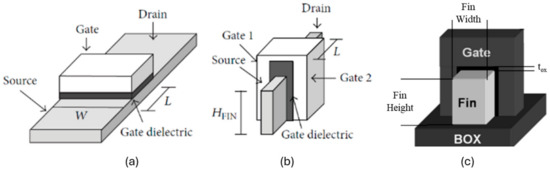
\includegraphics[scale=0.5]{assets/FinFET/FinFET-Overview.jpg}
			\caption{Structure Schematic of (a) planar MOSFET and (b) FinFET. (c) Demonstrating $H_{\symup{Fin}}$ as fin height and $W_{\symup{Fin}}$ as fin width. Taken from \cite{FinFET1}.}
			\label{fig:FinFET:FinFet-Overview}
		\end{figure}

	\subsection{Historical Development}

	To fully contextualize the introduction of FinFET technology, it is essential to review the key historical developments in semiconductor devices that preceded it. This progression illustrates the industry's response to escalating demands for miniaturization, speed, and power efficiency \cite{FinFET2}.\par

	The timeline of the modern electronics industry begins in 1904 with the launch of the vacuum tube \cite{FinFET2}. The vacuum tube, which controls the flow of electrons in a vacuum \cite{FinFET2}, served as the foundation of electronics for decades. However, it suffered from significant drawbacks, including diminished reliability, high power consumption, large physical size, and high manufacturing costs \cite{FinFET2}.\par

	The limitations of vacuum tubes led researchers to develop solid-state alternatives. A breakthrough occurred in 1947 with the construction of the point-contact transistor by William Shockley, John Bardeen, and Walter Brattain. This was followed in 1948 by William Shockley's invention of the Bipolar Junction Transistor (BJT) \cite{FinFET2}. These semiconductor devices proved to be far more reliable and power-efficient than vacuum tubes \cite{FinFET2}.\par

	A pivotal advancement in transistor technology occurred in 1956. During this period, M.M. Atalla addressed critical issues regarding semiconductor surfaces, identifying silicon dioxide as an effective solution for stabilization \cite{FinFET2}. This research led directly to the design of the Insulated-Gate Field Effect Transistor (IGFET), now universally known as the Metal-Oxide-Semiconductor Field-Effect Transistor (MOSFET) \cite{FinFET2}.\par

	The capacity for integration soon followed. In 1958, Jack Kilby developed the first integrated circuit (IC), which successfully joined several transistors on a single silicon substrate \cite{FinFET2}. The MOSFET proved exceptionally suitable for this high-density integration and became the driving engine of the digital world for over four decades \cite{FinFET2}.\par

	As device scaling continued, planar MOSFETs began to face significant challenges, such as short-channel effects. This necessitated a fundamental change in transistor architecture. This evolutionary path led to the fabrication of the first quasi-planar FinFET device in 2001 by N. Lindert et al., which was developed to suppress the DIBL (Drain-Induced Barrier Lowering) effect and enable further scaling \cite{FinFET2}.\par

	\subsection{FinFET Classifications}
	FinFET technology is not monolithic; rather, it encompasses several structural variations. These devices can be categorized based on three primary aspects: the substrate used, the gate terminal configuration, and the geometry of the dielectric.\break

	\subsubsection{Classification by Substrate}
	The first classification distinguishes FinFETs based on their fundamental physical structure and substrate. Bulk FinFETs, as illustrated in Figure \ref{fig:FinFET:class-substrate}(a) from the source material, are fabricated on a standard silicon substrate \cite{FinFET1}. In this configuration, the individual fins share a common substrate and are physically connected \cite{FinFET1}. This structure closely resembles that of traditional planar MOSFETs, which simplifies the manufacturing transition and integration process, leading many companies to prefer this approach \cite{FinFET1}. SOI (Silicon-on-Insulator) FinFETs, as Shown in Figure \ref{fig:FinFET:class-substrate}(b), are designed with physically isolated fins that sit atop a Buried Oxide (BOX) layer \cite{FinFET1}. This isolation from the silicon substrate provides distinct operational features \cite{FinFET1}. The choice between Bulk and SOI structures involves a complex engineering trade-off based on factors such as fabrication cost and specific performance requirements \cite{FinFET1}.

	\begin{figure}[h!]
			\centering
			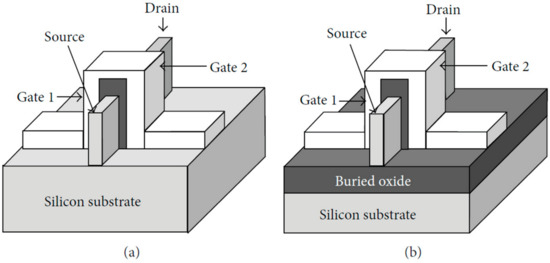
\includegraphics[scale=0.5]{assets/FinFET/fet-class-substrate.jpg}
			\caption{Structure schematic of (a) Bulk FinFET and (b) SOI FinFET \cite{FinFET1}.}
			\label{fig:FinFET:class-substrate}
	\end{figure}

	\subsubsection{Classification by Gate Type}
	The second classification is based on the number of terminals and the configuration of the gates, as shown in Figure \ref{fig:FinFET:class-gate} \cite{FinFET1}.
	Short Gate (SG) FinFETs are three-terminal devices where the two gates (Gate 1 and Gate 2) are physically connected, or "shorted," to each other \cite{FinFET1}. Independent Gate (IG) FinFETs are four-terminal devices. In this structure, the gates are physically isolated from one another by a dielectric material \cite{FinFET1}. This isolation allows for greater versatility, as varying voltages and signals can be applied to each gate terminal independently \cite{FinFET1}. IG FETs offer a superior $\nicefrac{I_{\symup{on}}}{I_{\symup{off}}}$ ratio because the voltage of one gate can be adjusted by the other, making them particularly well-suited for power management applications \cite{FinFET1}.

	\begin{figure}[h!]
		\centering
		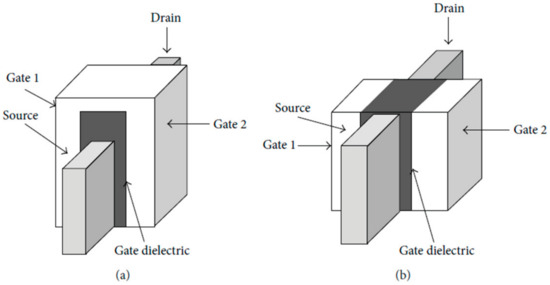
\includegraphics[scale=0.5]{assets/FinFET/fet-class-gate_type.jpg}
		\caption{Structure schematic of (a) SG FinFET and (b) IG FinFET. Taken from \cite{FinFET1}.}
		\label{fig:FinFET:class-gate}
	\end{figure}

	\subsubsection{Classification by Dielectric Geometry}
	The third classification, detailed in Figure \ref{fig:FinFET:class-dielectric} of the source, differentiates devices by the gate's coverage of the fin, which is determined by the dielectric thickness and geometry \cite{FinFET1}. In Double-Gate (DG) FinFET structure, a hard mask is employed on top of the fin. This effectively results in two gates, one on each vertical sidewall, with the top surface being non-conductive. The effective channel width is therefore calculated as two times the fin height \cite{FinFET1}. In a Tri-Gate FinFET configuration, the dielectric thickness on top of the fin is reduced, allowing the gate electrode to wrap over the top surface in addition to the two sidewalls \cite{FinFET1}. This creates a third gate, which enhances electrostatic control \cite{FinFET1}. Consequently, the total effective channel width for a Tri-Gate device is calculated as $(2 \times \text{fin height}) + \text{fin width}$ \cite{FinFET1}. This design offers distinct advantages, including lower gate-to-source capacitance and overall better performance, while maintaining strong electrostatic integrity \cite{FinFET1}.

	\begin{figure}[h!]
		\centering
		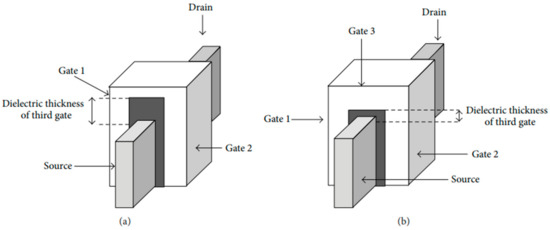
\includegraphics[scale=0.5]{assets/FinFET/fet-class-dielectric_geometry.jpg}
		\caption{Schematic of (a) DG FinFET and (b) tri-gate FinFET. Taken from \cite{FinFET1}.}
		\label{fig:FinFET:class-dielectric}
	\end{figure}

	\subsection{Materials in FinFET Fabrication}
	The performance, efficiency, and scalability of FinFET devices are critically dependent on the materials selected for their fabrication. Significant research has been directed toward optimizing materials for two key components: the gate dielectric and the channel.\par

	\subsubsection{Gate Dielectric Materials}
	A primary challenge in transistor scaling is the increase in gate leakage current as the traditional silicon dioxide ($\symup{SiO_2}$) dielectric layer becomes physically too thin \cite{FinFET1}. To counteract this, the industry has transitioned to high-k dielectric materials, which allow for a physically thicker layer while maintaining the same equivalent oxide thickness (EOT), thereby reducing leakage current \cite{FinFET1}. Hafnium Oxide ($\symup{HfO_2}$), for example, is a widely adopted high-k dielectric. Studies show that using $\symup{HfO_2}$ in a double-gate n-FinFET structure effectively reduces leakage current and offers significantly lower leakage than $\symup{SiO_2}$ \cite{FinFET1}.\par

	An even more cutting-edge high-k material is Lanthanum Zirconium Oxide ($\symup{LaZrO_2}$), which has a dielectric constant (k) of approximately 40, compared to 3.9 for $\symup{SiO_2}$ \cite{FinFET1}. As detailed in Table \ref{tab:gate-dielectrics}, its impact on device efficiency is substantial \cite{FinFET1}. When compared to $\symup{SiO_2}$ in an n-FinFET, $\symup{LaZrO_2}$ demonstrates a higher on-current ($I_{\symup{ON}}$) of $4.95 \times 10^{-5}$ A (versus $1.78 \times 10^{-5}$ A), a significantly lower off-current ($I_{\symup{OFF}}$) of $3.61 \times 10^{-14}$ A (versus $5.02 \times 10^{-13}$ A), and a dramatically improved $I_{\symup{ON}}/I_{\symup{OFF}}$ ratio of $1.37 \times 10^{9}$ (versus $3.50 \times 10^{7}$) \cite{FinFET1}. Furthermore, the $\symup{LaZrO_2}$ device shows a steeper Subthreshold Swing (SS) of 60.3 mV/dec and a much-reduced Drain-Induced Barrier Lowering (DIBL) effect of 10.1 mV/V, compared to 67.02 mV/dec and 43 mV/V for $\symup{SiO_2}$, respectively \cite{FinFET1}. These data confirm that high-k dielectrics are essential for enhancing electrostatic control, boosting the $I_{\symup{ON}}$/$I_{\symup{OFF}}$ ratio, and mitigating short-channel effects \cite{FinFET1}.\par

	\begin{table*}[]
	\centering
	\begin{tabular}{lll}
		\hline
		Parameters ($V_{\symup{d}}=0.75\unit{\volt}$, $V_{\symup{g}}=0.75\unit{\volt}$) & ($\symup{LaZrO}_{\symup{2}}$) Gate dielectric material $k = 40$ & ($\symup{SiO}_{\symup{2}}$) Gate dielectric material $k = 3.9$ \\
		\hline \hline
		$I_{\symup{ON}} (\unit{\ampere})$                            & $4.95 \times 10^{-5}$        & $1.78 \times 10^{-5}$        \\
		$I_{\symup{OFF}} (\unit{\ampere})$                           & $3.61 \times 10^{-14}$       & $5.02 \times 10^{-13}$       \\
		$\displaystyle\nicefrac{I_{\symup{ON}}}{I_{\symup{OFF}}}$    & $1.37 \times 10^{9}$         & $3.50 \times 10^{7}$         \\
		$V_{\symup{t}} (\unit{\volt})$                               & $0.253$                      & $0.207$                      \\
		SS $(\unit{{\milli\volt}\per{\decade}})$                     & $60.3$                       & $67.02$                      \\
		DIBL $(\unit{{\milli\volt}\per{\decade}})$                   & $10.1$                       & $43$                         \\
		\hline
	\end{tabular}
	\caption{The impact of $\symup{SiO_2}$ and $\symup{LaZrO_2}$ gate dielectric material usage in n-FinFET device efficiency.}
	\label{tab:gate-dielectrics}
\end{table*}

% For unit typesetting check https://www.tug.org/docs/latex/siunitx/siunitx.pdf

	\subsubsection{Channel Materials}
	In addition to dielectrics, optimization of the channel material is crucial. While silicon (Si) remains the dominant channel material, research into alternative materials has identified several candidates with superior properties for specific applications. For instance, in comparative simulations of SOI FinFET devices, 3C-SiC (Silicon Carbide) was found to exhibit the maximum $\nicefrac{I_{\symup{ON}}}{I_{\symup{OFF}}}$ ratio, calculated at $1.90 \times 10^{11}$, and the minimum $I_{\symup{OFF}}$ current, at $7.00 \times 10^{-19}\unit{\ampere}$ \cite{FinFET1}. Other materials, such as GaN (Gallium Nitride) and GaAs (Gallium Arsenide), are recognized for demonstrating superior DIBL characteristics, indicating better control over short-channel effects \cite{FinFET1}. Conversely, GaSb (Gallium Antimonide) has been identified as a poor-performing channel material, exhibiting the worst characteristics related to short-channel effects \cite{FinFET1}\par

	Looking forward, novel materials like Carbon Nanotubes (CNT) and Graphene are being investigated for their potential to significantly improve the $\nicefrac{I_{\symup{ON}}}{I_{\symup{OFF}}}$ ratio, increase operational speed, and reduce overall energy consumption in future FinFET devices \cite{FinFET1}. These material optimizations are part of a broad effort that also includes innovations like dual KK-structures for improving frequency response \cite{FinFET1}, InGaAs-on-Insulator for optimizing the on/off trade-off \cite{FinFET1}, and the use of Atomic Layer Deposition (ALD) for threshold voltage improvements \cite{FinFET1}.\par

	\subsection{Key Challenges in FinFET Technology}

	Despite their advantages over planar MOSFETs, the transition to FinFET technology introduces a unique set of fabrication and operational challenges. These must be addressed to optimize device performance and reliability.\par

	\subsubsection{Parasitic Capacitances}
	The three-dimensional nature of the FinFET, specifically the increased overlap region between the front and back gates, results in a higher incidence of parasitic capacitances compared to planar devices \cite{FinFET1}. As illustrated in Figure \ref{fig:FinFET:challenge-parasitic}, these capacitances exist between various terminals, such as gate-to-source/drain contacts (C2) and gate-to-source/drain diffusion (C3). This increased capacitance is a significant concern as it degrades the device's high-speed performance, leading to slower switching times \cite{FinFET1}.\par

	\begin{figure}[h!]
		\centering
		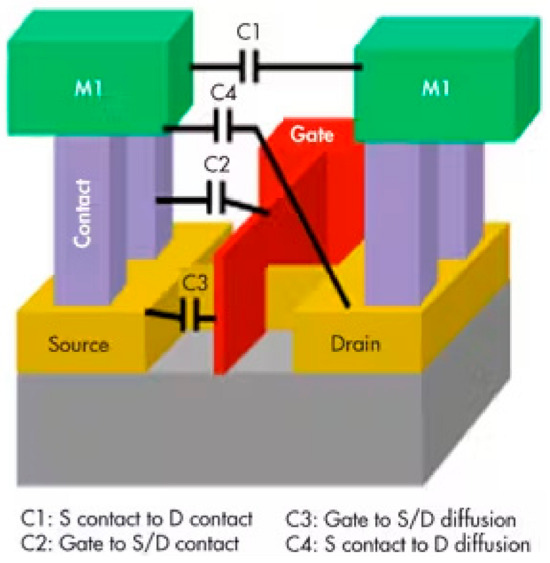
\includegraphics[width=0.5\linewidth]{assets/FinFET/fet-parasitic.jpg}
		\caption{Parasitic capacitances of a FinFET. Taken from \cite{FinFET1}.}
		\label{fig:FinFET:challenge-parasitic}
	\end{figure}

	\subsubsection{Corner Effects}
	A phenomenon unique to FinFETs is the ``corner effect''. While decreasing the fin width is effective for reducing short-channel effects, it can lead to a higher concentration of sub-threshold leakage current at the corners of the fin \cite{FinFET1}. This is due to enhanced electric fields at sharp edges \cite{FinFET1}. To mitigate this leakage path, FinFET production processes are modified to create fins with a more curved and rounded profile, as shown in the cross-sectional view in Figure \ref{fig:FinFET:challenge-corner} \cite{FinFET1}.\par

	\begin{figure}[h!]
		\centering
		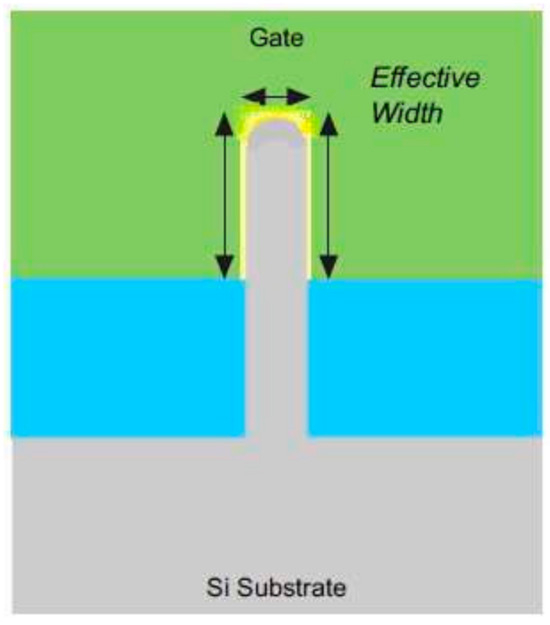
\includegraphics[width=0.5\linewidth]{assets/FinFET/fet-corner_effects.jpg}
		\caption{Cross-sectional view of a Tri-FinFET with curved fin corners. Taken from \cite{FinFET1}.}
		\label{fig:FinFET:challenge-corner}
	\end{figure}

	\subsubsection{Quantum Effects}\par
	As FinFETs scale to extremely thin fin widths, quantum mechanical effects become a significant performance limiter. In an ultra-thin fin, the density of available electron or hole states at the band edges diminishes \cite{FinFET1}. This ``quantum effect'' means that carriers (electrons or holes) require more energy to occupy states higher than the band edge before they can be liberated to conduct current \cite{FinFET1}. The practical result is a degradation of carrier mobility, which in turn reduces the drive current of the device.\par

	\subsubsection{Fabrication and Thermal Challenges}\par
	The fabrication of FinFETs is considerably more complex than that of planar MOSFETs. Creating the precise patterns for fins and gates demands an intricate level of process control, particularly in lithography \cite{FinFET1}. Furthermore, the narrow, tall structure of the fins poses thermal challenges. The smaller fin width, while beneficial for electrostatics, impedes the easy flow of heat out of the device, leading to an increase in device temperature \cite{FinFET1}. This phenomenon, known as self-heating, can negatively impact device reliability and performance.\par

	\subsection{Recent Innovations}
	To address the inherent challenges of FinFET technology, several structural innovations have been proposed to enhance performance and mitigate undesirable effects.

	The Ground-Plane FinFET (GP-FinFET), depicted in Figure \ref{fig:FinFET:innovation-gp}, introduces ground planes under the source and drain regions \cite{FinFET1}. This design was proposed to reduce the electric field coupling between the source and drain, thereby effectively minimizing Drain-Induced Barrier Lowering (DIBL) \cite{FinFET1}.\par

	\begin{figure}[h!]
		\centering
		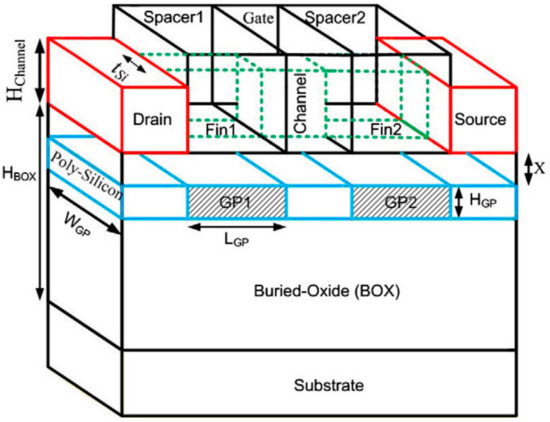
\includegraphics[width=0.6\linewidth]{assets/FinFET/finfet-gp.jpg}
		\caption{Three-dimensional view of the GP-FinFET structure schematic. Taken from \cite{FinFET1}.}
		\label{fig:FinFET:innovation-gp}
	\end{figure}

	A second innovation is the Bottom-Spacer (BS) FinFET, shown in Figure \ref{fig:FinFET:innovation-bs}. This structure was conceived to improve short-channel effect and self-heating performance \cite{FinFET1}. It incorporates an added spacer region that insulates the inactive (lower) portion of the fin from the gate contact, leading to improved control over short-channel effects and better thermal management \cite{FinFET1}.

	\begin{figure}[h!]
		\centering
		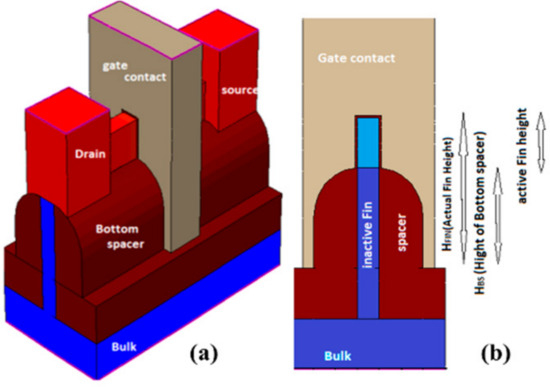
\includegraphics[width=0.7\linewidth]{assets/FinFET/finfet-bottom_spacer.jpg}
		\caption{(a) 3D view and (b) side view of the structure of bottom spacer FinFET. Taken from \cite{FinFET1}.}
		\label{fig:FinFET:innovation-bs}
	\end{figure}

	Finally, the Negative Capacitance FinFET with Ferroelectric Spacer (NCFS), illustrated in Figure \ref{fig:FinFET:innovation-ncfs}, employs a ferroelectric material in the spacer region rather than a traditional dielectric \cite{FinFET1}. The polarization of this ferroelectric material amplifies the electric field, which leads to enhancements in key performance metrics, including a higher on-state current ($I_{\symup{on}}$) and a lower, or steeper, subthreshold slope (SS) \cite{FinFET1}.

	\begin{figure}[h!]
		\centering
		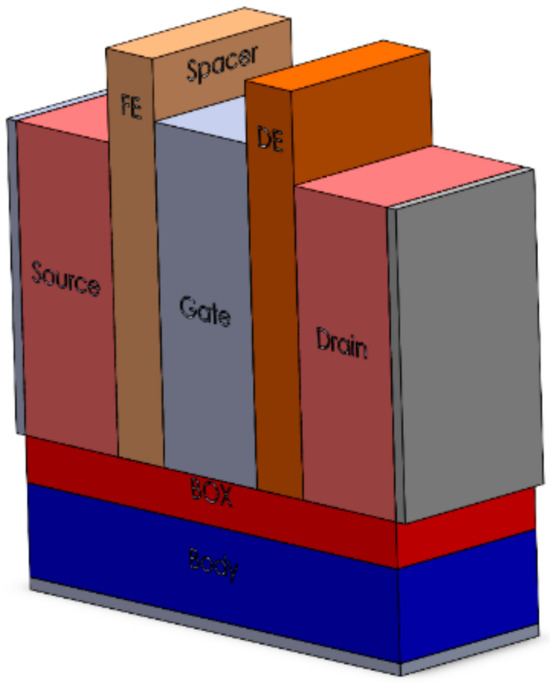
\includegraphics[width=0.45\linewidth]{assets/FinFET/finfet-negative_capacitance.jpg}
		\caption{Three-dimensional view of the most effective structure of Negative Capacitance FinFET with Ferroelectric Spacer. Taken from \cite{FinFET1}.}
		\label{fig:FinFET:innovation-ncfs}
	\end{figure}

	\subsection{Multi-Fin FinFET}

	A prevalent industry-standard implementation of the FinFET architecture is the Multi-Fin FinFET (M-FinFET). As illustrated in Figure \ref{fig:FinFET:n-finfet}, this design methodology positions multiple ``fins'', or channels, in parallel between the source and drain terminals \cite{FinFET2}.\par

	The primary advantage of this configuration is its ability to allow a higher number of charge carriers to traverse the device from source to drain simultaneously. This capability for increased current flow directly results in enhanced operational speed for the device \cite{FinFET2}.

	\begin{figure}[h!]
		\centering
		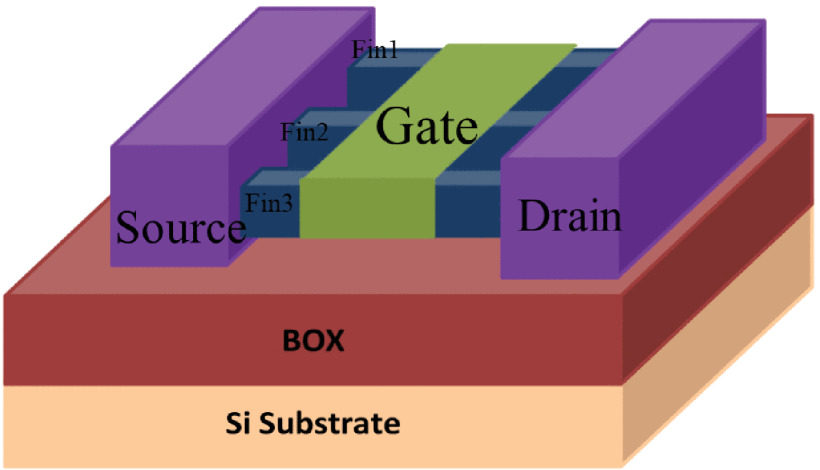
\includegraphics[scale=0.15]{assets/FinFET/m-finfet.jpg}
		\caption{Schematic diagram of M-FinFET. Taken from \cite{FinFET2}.}
		\label{fig:FinFET:n-finfet}
	\end{figure}

	\subsection{Motivation: Limitations of Planar MOSFETs}
	The development of FinFET technology was motivated by the fundamental limitations of traditional planar MOSFETs, as depicted in Figure \ref{fig:FinFET:mosfet}. As device scaling progressed to dimensions below $32\unit{\nano\meter}$, planar transistors began to exhibit significant performance issues \cite{FinFET2}.

	\begin{figure}[h!]
		\centering
		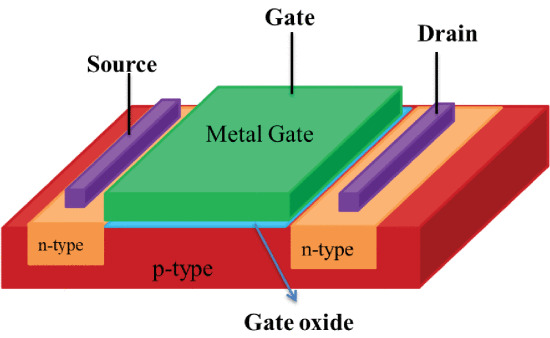
\includegraphics[scale=0.25]{assets/FinFET/planar-fet.jpg}
		\caption{The planar MOSFET semiconductor device. Taken from \cite{FinFET2}.}
		\label{fig:FinFET:mosfet}
	\end{figure}

	These issues include strong short-channel effects (SCE), a substantial increase in leakage currents, and greater threshold voltage variation \cite{FinFET2}. Such problems arise because the single gate of a planar device loses electrostatic control over the channel at small scales \cite{FinFET2}. This weak gate control leads to poor electrostatic integrity and significant power inefficiency.\par

	To overcome these scaling barriers, a new architecture was required\cite{FinFET2}. This necessitated the move to multi-gate structures (MuGFETs), such as the FinFET shown in Figure \ref{fig:FinFET:finfet-normal}, to re-establish strong gate control over the channel\cite{FinFET2}.

	\begin{figure}[h!]
		\centering
		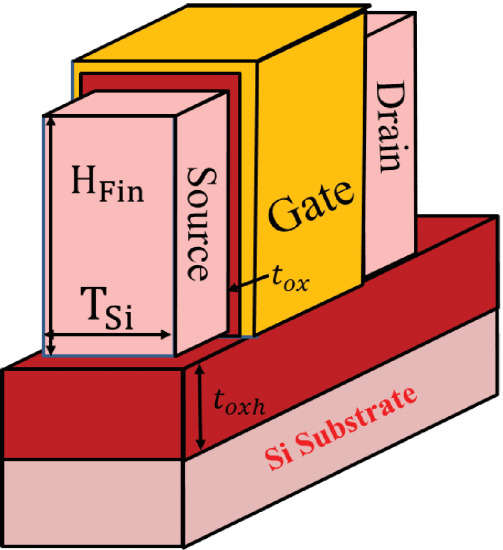
\includegraphics[scale=0.15]{assets/FinFET/fet-normal.jpg}
		\caption{Schematic diagram of conventional FinFET. Taken from \cite{FinFET2}.}
		\label{fig:FinFET:finfet-normal}
	\end{figure}


	\subsection{Conclusion: The Next Generation}

	FinFET technology has been instrumental in continuing semiconductor advancement, providing a scalable, low-power solution that has extended down to the $5\unit{\nano\meter}$ node \cite{FinFET1}. However, as FinFETs approach their physical scaling limits, they face persistent challenges in areas such as thermal management \cite{FinFET2} and manufacturing cost and complexity \cite{FinFET1}.\par

	To overcome these barriers and enable further miniaturization, the industry is transitioning to the next evolutionary architecture: the Gate-All-Around (GAA) FET \cite{FinFET2}. As illustrated in Figure \ref{fig:FinFET:fet-gaa}, the GAA structure offers superior electrostatic control by enveloping the channel from all sides, a critical requirement for nodes below $5\unit{\nano\meter}$.\par

	This transition from FinFET to GAA is not merely a future prospect; it is the industry's current trajectory. Samsung has been a pioneer in this shift, having introduced its first-generation $3\unit{\nano\meter}$ GAA MBCFET chips in 2022 \cite{FinFET2}\cite{FinFET3-samsung}. Meanwhile, Intel is introducing its GAA-based ``RibbonFET'' technology around 2026 \cite{FinFET4-intel}, and TSMC is de-veloping its $2\unit{\nano\meter}$ GAA platform for a target launch also around 2026 \cite{FinFET5-tsmc}. This clear industry-wide pivot confirms that the GAA architecture is succeeding the FinFET as the new standard to enable the future of semiconductor technology.

	\begin{figure}[h!]
		\centering
		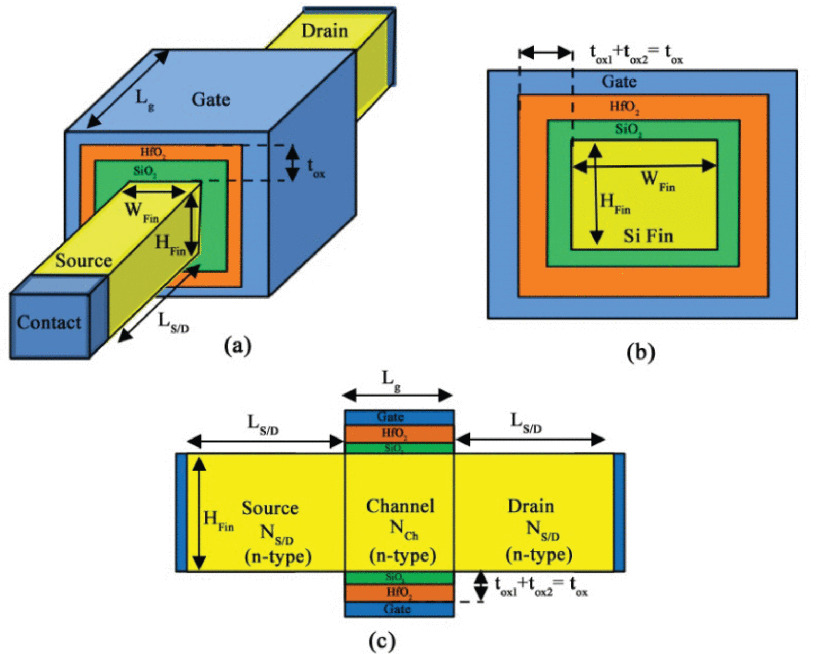
\includegraphics[width=0.75\linewidth]{assets/FinFET/GAA-FET.jpg}
		\caption{Schematic diagram of GAA structure along (a) Vertical (b) and horizontal view (c). Taken from \cite{FinFET2}.}
		\label{fig:FinFET:fet-gaa}
	\end{figure}

	\section{Fully Depleted-Silicon on Insulator (FD-SOI)}\label{section:FDSOI}

	\subsection{Technology overview}
		MOSFET scaling, need for power consumption reduction, and short-channel effects (SCEs) (due to scaling) led to exploration of new planar architectures. One such structure tackling the above is silicon on insulator (SOI) \cite{Fossum_Trivedi_2013}\cite{FDSOICMOS}. Fully depleted-silicon on insulator (FD-SOI) devices are a subclass of SOI devices \cite{Fossum_Trivedi_2013}\cite{FDSOICMOS}. SOI devices consist of a silicon layer on top of a silicon oxide called \textsl{burried oxide} (BOX) --formed as a single crystal-- and a Si substrate beneath the BOX \cite{FDSOICMOS}.\par

		The Si-film beneath the gate --often referred to as \textsl{body}-- is depleted of free carriers; hence, the name \textsl{fully depleted-silicon on insulator} \cite{Fossum_Trivedi_2013}\cite{FDSOICMOS}\cite{NYSSENS202433}. Figure \ref{fig:FDSOI:CMOS} shows the cross-section of a CMOS pair on p-substrate in $28\unit{\nano\meter}$ UTBB FD-SOI CMOS process, where insulator is used to isolate nMOSFETS from pMOSFETS. UTBB stands for \textsl{ultra-thin body and BOX} \cite{NYSSENS202433}. This specific version of FD-SOI offers additional control over the threshold voltage, $V_{\symup{th}}$, through the biasing of the doped silicon layer (\textsl{well} \cite{7469814} or \textsl{ground-plane} \cite{nazarov_functional_2014}) beneath the box \cite{NYSSENS202433}. The terminal controlling the well beneath the BOX is called \textsl{back-gate} (BG) \cite{NYSSENS202433}.\par

		\begin{figure}[h!]
			\centering
			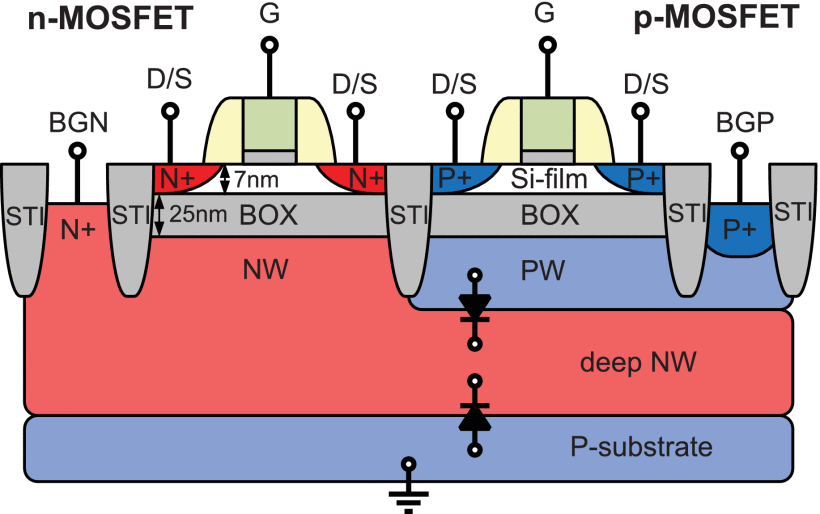
\includegraphics[width=0.7\linewidth]{assets/FD-SOI/FD-SOI_CMOS.png}
			\caption{Cross-section of the n- and p-channel MOSFETs with back-gate wells and deep n-well in $28\unit{\nano\meter}$ UTBB FD-SOI CMOS process. Taken from \cite{7469814}.}
			\label{fig:FDSOI:CMOS}
		\end{figure}
		One key advantage of FD-SOI devices is their reduced junction capacitance \cite{NYSSENS202433}. The drain junction capacitance, $C_{dj}$, can be decomposed into two capacitances: a vertical capacitance between the drain and the substrate, $C_{djv}$, and a lateral capacitance between the drain and the body of the MOSFET, $C_{jdl}$, \cite{FDSOICMOS}. Because the body is usually thin, especially in UTBB processes, $C_{jdl}$ is small \cite{FDSOICMOS}. Moreover, $C_{djv}$ is small thanks to the BOX and therefore, the total drain junction capacitance, $C_{dj}$, is small compared to that of bulk-Si and it is hardly affected by variations in the drain voltage \cite{FDSOICMOS}. Hence, the physical isolation of the active device from the substrate reduces junction capacitance enabling greater speeds and operation in lower voltages \cite{FDSOICMOS} which is crucial to reduction in power dissipation.\par

		Additionally, FD-SOI devices exhibit a steeper subthreshold slope than bulk-Si \cite{FDSOICMOS}. A steeper subthreshold characteristic ($\log{\left( I_d \right)}$ vs $V_{g}$) means that at $V_{g}=0\unit{\volt}$ the leakage current will be significantly lower \cite{FDSOICMOS}. This is, partially, attributed to the isolation of the \textsl{active device} from the well trhough the BOX \cite{NYSSENS202433}.\par

		In FD-SOI it is possible to lower the threshold voltage \cite{FDSOICMOS}; one way is through applying voltage bias to the back-gate of ultra-thin body (UTB) FD-SOI devices \cite{Fossum_Trivedi_2013}. According to \cite{FDSOICMOS}, the propagation delay time, $\tau$, in CMOS VLSI is inversely proportional to the square of the difference between the supply voltage, $V_{\symup{DD}}$, and the threshold voltage, $V_{\symup{th}}$. That is $\tau\propto\nicefrac{1}{\left( V_{\symup{DD}} - V_{\symup{th}} \right)^2}$. Hence, lowering the threshold voltage decreases the propagation delay time.\par

		\cite{nazarov_functional_2014} and \cite{FDSOICMOS} report high transconductance-to-drain-current ratio, $\nicefrac{g_m}{I_d}$, values compared to bulk-Si, especially for smaller channel lengths. Furthermore, \cite{FDSOICMOS} claims sufficiently high output resistance, $r_{ds}=g_{ds}^{-1}$, for FD-SOI devices. Hence, the intrinsic voltage gain of FD-SOI devices $$A_v=\frac{g_m}{g_{ds}}=\frac{g_m}{I_d}V_{\symup{Early}},$$ where $V_{\symup{Early}}=\nicefrac{I_d}{g_{ds}}$ is the Early voltage, is high making it ideal for analog applications \cite{nazarov_functional_2014}. Taking into consideration the gain bandwidth product expression $$\symup{GBW}=\frac{g_m}{I_d}\cdot\frac{I_d}{2\pi C_L},$$ where $C_L$ represents a capacitive load, it is easy to see that it increases since $A_v$ increases.\par

		DIBL can be minimized utilizing the back-gate \cite{FDSOICMOS}. Applying a back-gate bias the formation of a back-channel, beneath the BOX, is avoided \cite{FDSOICMOS}. \cite{5703287} showcases much lower DIBL for FD-SOI (Si film thickness, $t_{\symup{Si}}$, between $7\unit{\nano\meter}$ and $9\unit{\nano\meter}$) than bulk-Si and comparable DIBL to FinFETs.

	\subsection{1T-APS}

The authors of \cite{FDSOI1} propose an active pixel sensor (APS) comprised of a single transistor. The device is fabricated using 22-nm FD-SOI technology and it is tested with light of wavelength of $520\unit{\nano\meter}$ \cite{FDSOI1}. The proposed sensor belongs to a class of devices referred to as \textsl{charge-coupled devices} (CCD) \cite{FDSOI1}.\par
CCD-based sensors take advantage of electrical charge accumulated during measurements \cite{CCD}. Later, the charge is transformed into voltage or current, amplified and measured \cite{CCD}. The proposed device is shown in figure \ref{fig:FDSOI:TEM}.\par
Traditional CMOS pixel sensors consist of a photodiode with four auxiliary transistors \cite{FDSOI1}\cite{1715616}. The proposed pixel integrates the photodiode, the reset function, and the signal amplification in a single device. Beneath the box there is an n-well on a p-substrate. This pn junction acts as the photodiode \cite{FDSOI1}.\par

\begin{figure}[h!]
	\centering
	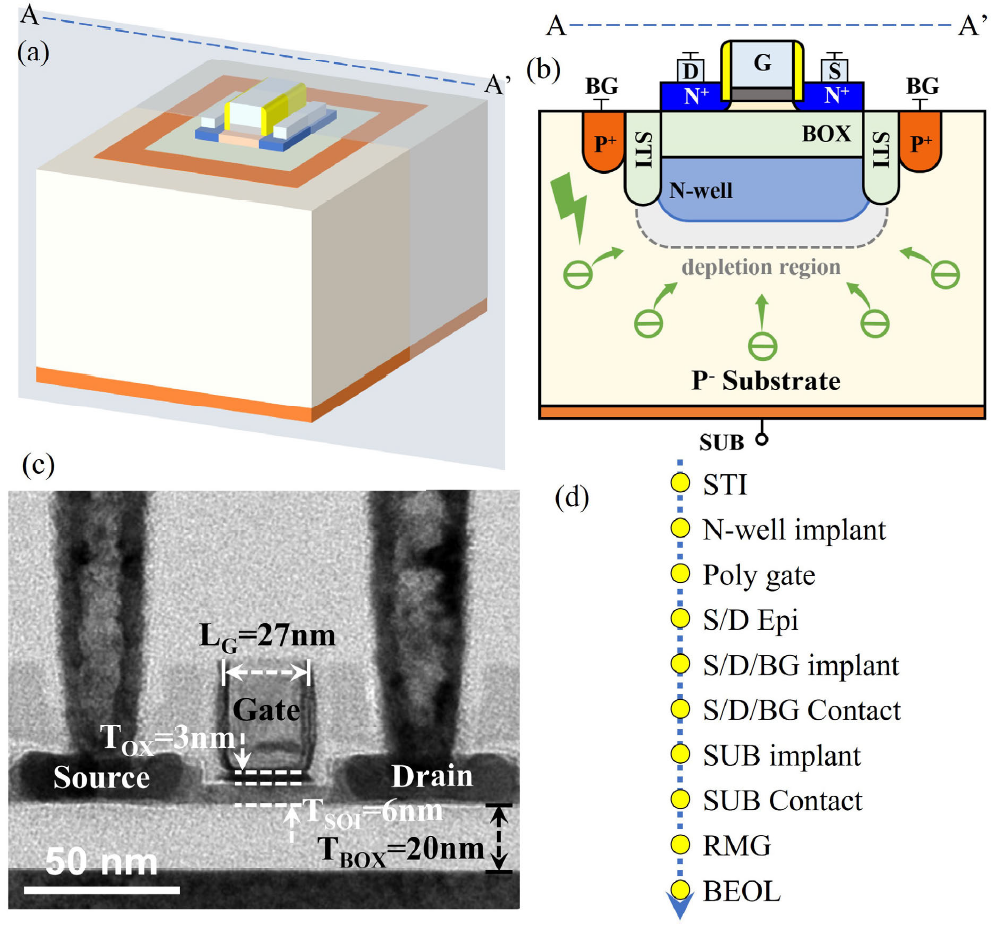
\includegraphics[width=0.9\linewidth]{assets/FD-SOI/1T_Pixel_Sensor/TEM.png}
	\caption{ (a) Schematic 3D structure and (b) 2D cross-section of 1T-APS. (c) XTEM image and (d) the simplified process flow. Taken from \cite{FDSOI1}.}
	\label{fig:FDSOI:TEM}
\end{figure}

\subsubsection{Operation}

	A negative voltage pulse is applied to the substrate (SUB) and back-gaet (BG) electrodes. This pulse leads to the formation of a depletion region on the pn junction as shown in figure \ref{fig:FDSOI:TEM} \cite{FDSOI1}. In the experiments performed by the authors, light of wavelength $\lambda=520\unit{\nano\meter}$ (green visible light) was used. When light hits the photodiode charges start to accumulate causing a variation of drain current, $I_d$, \cite{FDSOI1}. $I_d$ can be amplified, if needed, and measured to obtain the response of the sensor.\par
	The authors verified experimentally the successful reset of the sensor by zeroing the voltage at the SUB and BG electrodes and reapplying negative pulses to the same terminals \cite{FDSOI1}.\par
	It is demonstrated that the potential of the substrate is mainly controlled by the back-gate (BG) terminal \cite{FDSOI1}. Additionally, $V_{bg}$ controls the size of the depletion area \cite{FDSOI1}; thus, affecting the full-well capacity (FWC). Full-well capacity is a means of quantifying the total charge that can be stored in the photodiode well \cite{LEE2022108472}; i.e. beneath the BOX in this case. Hence, $V_{bg}$ and $V_{sub}$ can be used as tuning knobs for the sensor sensitivity \cite{FDSOI1}.\par

	\begin{figure}[h]
		\centering
		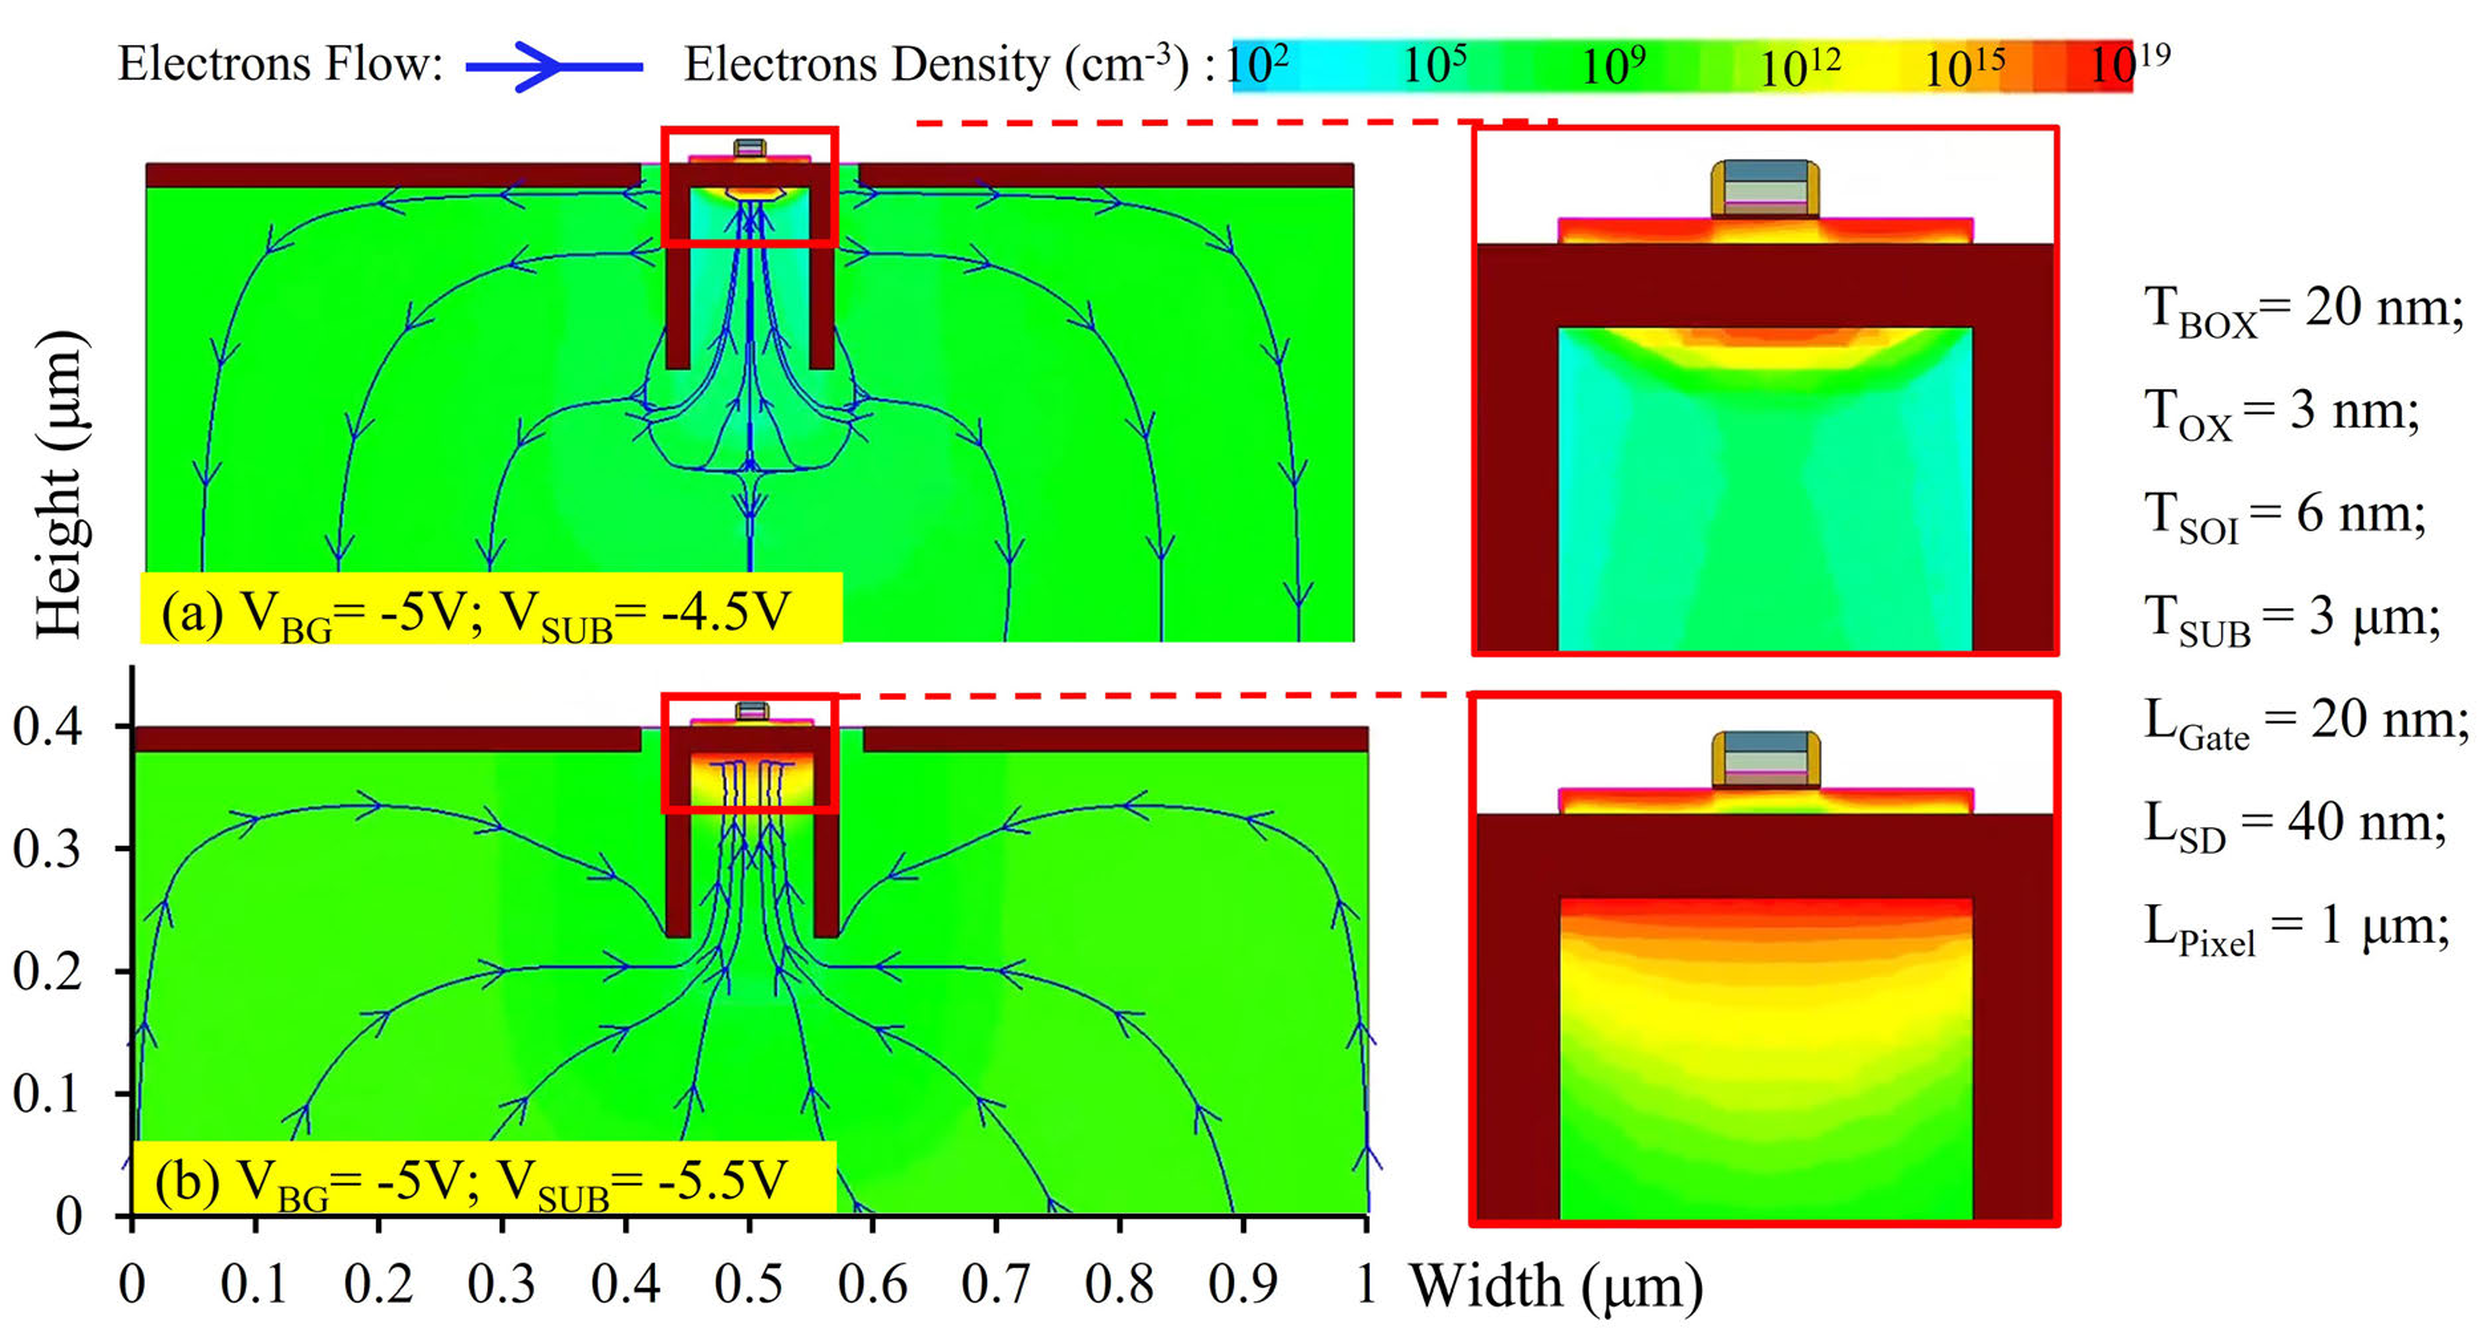
\includegraphics[width=0.9\linewidth]{assets/FD-SOI/1T_Pixel_Sensor/electrostatics.png}
		\caption{On the left: electron flow during exposure. On the right: electron distribution during exposure. Taken from \cite{FDSOI1}.}
		\label{fig:fdsoi:pixel:electrostatics}
	\end{figure}

	Figure \ref{fig:fdsoi:pixel:electrostatics} shows how the potential difference $V_{bg}-V_{sub}$ affects the flow of electrons from the substrate toward or away from the area beneath the BOX; hence, there is difference in the sensor's sensitivity \cite{FDSOI1}. $V_{bg}\lneqq V_{sub}$ forces the substrate-electrons away from the well beneath the BOX \cite{FDSOI1}. On the other hand, $V_{bg}\gneqq V_{sub}$ pushes electrons toward the well increasing the accumulated charge and increasing sensitivity \cite{FDSOI1}.\par

	\subsection{Sub $6\unit{\giga\hertz}$ transceiver front-end in $22$-$\unit{\nano\meter}$ FD-SOI CMOS}

	The final article discussed, \cite{FDSOI2}, proposes a highly integrated sub-$6\unit{\giga\hertz}$ --specifically, $f_{\symup{RF}}\in \left[ 1.25\unit{\giga\hertz}, 5.5\unit{\giga\hertz} \right]$-- tranceiver (TRx) front-end for cellular base stations. The IC is fabricated using 22nm FD-SOI technology. In order to meet the application requirements while using on-chip power amplifiers, the authors chose to use a $12.5\unit{\ohm}$ impedance. The advantage of using a low impedance is that it allows for low-voltage power amplification, since $P_{\symup{diss}}={V^2}{Z^{-1}}$. However, low input impedance --in the Rx front-end-- reduces the input voltage; hence, the targeted noise figure is harder to reach and a higher supply voltage is needed for the LNA \cite{FDSOI2}. The proposed IC is shown in figure \ref{fig:FDSOI:TRX:system}.\par

	The integrated part of the transmitter (Tx) consists of two pre-power-amplifier (PPA1 and PPA2) stages with variable gain and a power amplifier (PA). Additionally, the RF input signal is translated to baseband, filtered through a low-pass filter (LPF) and it is translated again to $f_{\symup{RF}}$ before it is substracted from the output signal of the first pre-power-amplifier stage (PPA1); the LP filter is in parallel to PPA1 (see figure \ref{fig:FDSOI:TRX:system}). The LPF is necessary for suppressing any intermodulation products that occur from the RF digital to analog converter's (DAC) clock --preceding PPA1 and not shown in figure \ref{fig:FDSOI:TRX:system}-- and the signals \cite{FDSOI2}.

	The integrated part of the receiver (Rx) consists of a low noise amplifier (LNA), followed by a variable gain amplifier (VGA), a three-frequency-band equalizer and finally a buffer. There is also a switch connected to the antenna array used for enabling either the Tx or Rx.\par

	It is important to note that both the Rx and Tx feature no frequency translation (except for the LPF); hence, all the amplifiers require wide bandwidth. Finally, all amplifiers in figure \ref{fig:FDSOI:TRX:system} are fully differential.\par

	\begin{figure}[htb]
		\centering
		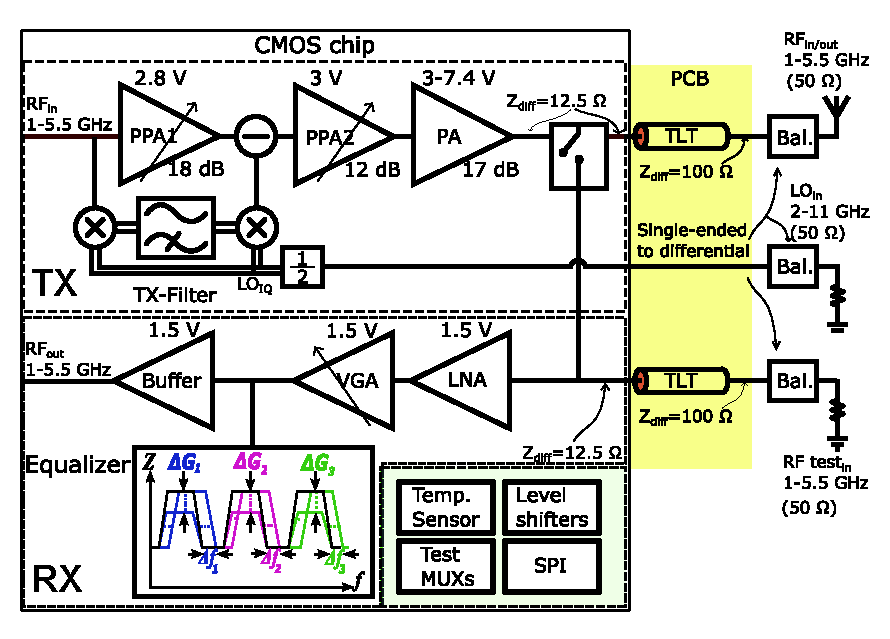
\includegraphics[width=\linewidth]{assets/FD-SOI/Sub_6GHz_TRX_assets/system.pdf}
			\caption{Simplified schematic of the proposed integrated tranceiver \cite{FDSOI2}.}
		\label{fig:FDSOI:TRX:system}
	\end{figure}

	\subsubsection{Noise factor} To better understand device-related noise, a means to quantify the device-added noise is needed. Let $G$ be the gain of an amplifier, $\symcal{S}_{\symup{in}}$, $\symcal{S}_{\symup{out}}$, $\symcal{N}_{\symup{in}}$ and $\symcal{N}_{\symup{out}}$ the power of the input signal, the power of the output signal, the power of the input noise and the power of the output noise, respectively. The ratio of the input SNR (signal-to-noise ratio), $\symup{SNR}_{\symup{in}}$, to the output SNR, $\symup{SNR}_{\symup{out}}$, is called \textsl{noise factor}.
	\begin{equation}
		\label{eq:noise_factor_definition}
		\symup{F}=\frac{\symup{SNR}_{\symup{in}}}{\symup{SNR}_{\symup{out}}}
	\end{equation}
	However, in practice \textsl{noise figure} is preferred over noise factor for characterizing a device. Noise figure, $\symup{NF}$, is the noise factor expressed in decibels; $\symup{NF}=10\log_{10}{\left(\symup{F}\right)}$ \cite{frenzel2015principles}.

	Some of the most prominent sources of device-added noise are resistors (thermal noise) and active devices \cite{RFICRogers}. We will prove that the noise factor of any real device is greater than unity. To do this we begin from the definition of noise factor in equation \eqref{eq:noise_factor_definition}.
	\begin{align*}
		& \symup{F} = \frac{\symup{SNR}_{\symup{in}}}{\symup{SNR}_{\symup{out}}} \Rightarrow\\
		& \symup{F} = \frac{\symcal{S}_{\symup{in}}}{\symcal{N}_{\symup{in}}} \cdot \frac{\symcal{N}_{\symup{out}}}{\symcal{S}_{\symup{out}}} \Rightarrow\\
		& \symup{F} = \frac{\symcal{S}_{\symup{in}}}{\symcal{N}_{\symup{in}}} \cdot \frac{G\cdot \symcal{N}_{\symup{in}} + \symcal{N}_{\symup{device}}}{G\symcal{S}_{\symup{in}}} \Rightarrow\\
		& \symup{F} = 1 + \frac{\symcal{N}_{\symup{device}}}{G\cdot \symcal{N}_{\symup{in}}} \gneqq 1,
	\end{align*}
	since $\symcal{N}_{\symup{device}}\gneqq 0$ for all real devices.

	\subsubsection{Low noise amplifier (LNA)}

		Low noise amplifiers (LNAs) are quite often the first component, after the antenna, in the Rx chain and that is because the noise figure/factor of the first subsystem dominates the system's total noise figure/factor \cite{frenzel2015principles}. This is apparent in the expression of the noise factor of system comprising of $N$ cascaded subsystems, each with gain $G_j$:
		\begin{equation}
			\label{eq:cascode_noise_factor}
			F_{\symup{tot}}=F_1+\sum_{i=2}^{N}{\frac{F_i-1}{\prod_{j=1}^{i-1}{G_j}}}
		\end{equation}

		\begin{figure}[ht!]
			\centering
			\begin{tikzpicture}
	% Paths, nodes and wires:
	\draw (-2.98, 3.27) -- (-2.48, 3.27);
	\draw (-1.5, -0.04) -- (-1.5, -0.29);
	\draw (1.5, -0.04) -- (1.5, -0.29);
	\path[draw={rgb,255:red,63;green,63;blue,63}, dash pattern={on 1.6pt off 1.6pt}, latex-latex] (-2.625, 1.21) -- (-0.75, 0.335);
	\node[nmos, arrowmos, xscale=-1](N1) at (-2.98, -0.04){} node[anchor=east] at (N1.text){$\symup{M}_{11}$};
	\node[nmos, arrowmos](N2) at (2.98, -0.04){} node[anchor=west] at (N2.text){$\symup{M}_{12}$};
	\node[nmos, arrowmos](N3) at (2.98, 2.5){} node[anchor=west] at (N3.text){$\symup{M}_{22}$};
	\node[nmos, arrowmos, xscale=-1](N4) at (-2.98, 2.5){} node[anchor=east] at (N4.text){$\symup{M}_{21}$};
	\draw (-2, 2.5) -- (2, 2.5);
	\node[vcc](N5) at (0, 4.5){} node[anchor=south] at ([yshift=-0.12cm]N5.text){$V_{\symup{DD}}$};
	\draw (-2, -0.04) to[cute inductor, inductors/width=1.5, inductors/coils=10, l_={$L_g$}] (2, -0.04);
	\node[ocirc](N6) at (-1.5, -0.29){} node[anchor=north] at ([yshift=0.04cm]N6.south){$v_{\symup{in}^{+}}$};
	\node[ocirc](N7) at (1.5, -0.29){} node[anchor=north] at ([yshift=0.04cm]N7.south){$v_{\symup{in}^{-}}$};
	\node[circ, yscale=-1] at (-0, 0.17){};
	\node[circ] at (-1.5, -0.04){};
	\node[circ] at (1.5, -0.04){};
	\draw (-0, -1.54) to[cute inductor, l={$L_{\symup{deg}}$}] (-0, -2.54);
	\draw (-2.98, -0.81) |- (-2.75, -1.29) -- (2.5, -1.29) -| (2.98, -0.81);
	\draw (-0, -1.54) -| (-0, -1.29);
	\node[circ] at (-0, -1.29){};
	\draw (-0, -2.54) -| (-0, -2.79);
	\node[tlground] at (-0, -2.79){};
	\node[tlground] at (-0, -2.79){};
	\draw (-2.98, 1.73) to[cute inductor, l_={$L_{dl}$}] (-2.98, 0.73);
	\node[circ, xscale=0.75, yscale=0.75] at (-2.625, 0.835){};
	\node[circ, xscale=0.75, yscale=0.75] at (-1.125, 0.335){};
	\draw (2.98, 0.73) to[cute inductor, l_={$L_{dr}$}] (2.98, 1.73);
	\node[circ, xscale=-0.75, yscale=-0.75] at (2.625, 1.625){};
	\path[draw={rgb,255:red,63;green,63;blue,63}, dash pattern={on 1.6pt off 1.6pt}, latex-latex] (-2.625, 1.585) -- (2.5, 1.585);
	\node[shape=rectangle, fill={rgb,255:red,255;green,255;blue,255}, minimum width=0.34cm, minimum height=0.235cm](N8) at (-0, 1.595){} node[anchor=center] at (N8.text){\textcolor{rgb,255:red,63;green,63;blue,63}{$k_2$}};
	\node[shape=rectangle, fill={rgb,255:red,255;green,255;blue,255}, minimum width=0.34cm, minimum height=0.34cm](N9) at (-1.688, 0.773){} node[anchor=center] at (N9.text){\textcolor{rgb,255:red,63;green,63;blue,63}{$k_1$}};
	\path[draw={rgb,255:red,63;green,63;blue,63}, dash pattern={on 1.6pt off 1.6pt}, latex-latex] (0.75, 0.335) -- (2.625, 1.21);
	\node[shape=rectangle, fill={rgb,255:red,255;green,255;blue,255}, minimum width=0.34cm, minimum height=0.34cm](N10) at (1.688, 0.773){} node[anchor=center] at (N10.text){\textcolor{rgb,255:red,63;green,63;blue,63}{$k_1$}};
	\node[ocirc](N11) at (-2.48, 3.27){} node[anchor=west] at ([xshift=-0.04cm]N11.east){$v_{\symup{out}^{-}}$};
	\node[circ] at (-2.98, 3.27){};
	\draw (2.48, 3.27) -- (2.98, 3.27);
	\node[ocirc](N12) at (2.48, 3.27){} node[anchor=east] at ([xshift=0.04cm]N12.west){$v_{\symup{out}^{+}}$};
	\node[circ] at (2.98, 3.27){};
	\draw (-1.25, 4.29) to[cute inductor, inductors/width=1.5, inductors/coils=10, l_={$L_{\symup{out}}$}] (1.25, 4.29);
	\draw (2.98, 3.27) |- (1.25, 4.29);
	\draw (-2.98, 3.27) |- (-1.25, 4.29);
	\node[circ] at (0, 4.5){};
	\node[circ] at (-0, 2.5){};
	\node[vcc](N13) at (-0, 0.17){} node[anchor=south] at ([yshift=-0.12cm]N13.text){$V_{\symup{CS}}$};
	\node[vcc](N14) at (0, 2.5){} node[anchor=south] at ([yshift=-0.12cm]N14.text){$V_{\symup{CG}}$};
\end{tikzpicture}
			\caption{LNA schematic with transformer feedback presented in \cite{FDSOI2}. $\symup{M}_{11}$ and $\symup{M}_{12}$ are identical. $\symup{M}_{21}$ and $\symup{M}_{22}$ are identical.}
			\label{fig:FDSOI:TRX:LNA}
		\end{figure}

		The noise factor of cascode MOSFET pair, where the transistor in common-source (CS) topology acts as the input transistor, is inversely proportional to the input transistor's transconductance, $g_{m,\symup{CS}}$, \cite{Adaptive2008}. Hence, the noise factor can be reduced by increasing the input transconductance \cite{FDSOI2} \cite{Adaptive2008}. The LNA schematic of \cite{FDSOI2} is shown in figure \ref{fig:FDSOI:TRX:LNA}. It is a fully differential amplifier; that is both the input and output are differential. The input comprises of a CS differential pair of nMOSFETs and the output comprises of a common gate (CG) differential pair of nMOSFETs.\par

		The cascode transistors, $\symup{M}_{21}$ and $\symup{M}_{22}$, improve isolation between the input and output ports of the amplifier \cite{RFICRogers}. In order to synthesize a real impedance at the output node of the LNA an inductor, $L_{\symup{out}}$, is placed between the node and the voltage supply, $V_{\symup{DD}}$. $L_{\symup{out}}$ resonates, at a specific frequency, with the total equivalent capacitance at the output node introduced by $\symup{M}_{2x}$; hence, matching with the following stage  in the Rx chain is achieved.\par
		Two important techniques are used by the authors of \cite{FDSOI2}; the first one is \textsl{reactive series-shunt feedback} and the second one is \textsl{source degeneration}. Both of these techniques are explained in detail in the following paragraphs.\par

		\textbf{Source degeneration.}
	Consider an nMOS common source (CS) amplifier. The input of this amplifier is connected to the output of a system with output impedance $\symbb{R}\ni Z_0=R_0+j0$. In order to match the input impedance of the CS amplifier to $Z_0$, it is common to use two inductors \cite{CMOSRFIC}; one at the input of the CS amplifier, $L_G$, and one at the source of the nMOS, $L_S$ \cite{CMOSRFIC}. This technique is called \textsl{source degeneration} \cite{CMOSRFIC}. The inductive pair $L_G + L_S$ is used to resonate --at a specific frequncy, $\omega_T$-- the gate-source capacitance of the transistor, $C_{gs}$, and $L_S$ is used to bring the value of the input impedance closer to $Z_0$ \cite{CMOSRFIC}.\par

	\cite{FDSOI2} uses source degeneration when the amplifier works in common mode \cite{FDSOI2} --that is when $v_{\symup{in}^{+}} = v_{\symup{in}^{-}}$-- in order to reduce common-mode gain. In this case, the voltage drop across $L_g$ is zero and a small-signal equivalent of the CS amplifier (figure \ref{fig:FDSOI:TRX:LNA:SOURCE_DEG:initial}) is shown in figure \ref{fig:FDSOI:TRX:LNA:SOURCE_DEG:equiv}. Assuming both transistors to be identical, the input impedance can be calculated as follows.

	\begin{figure}[h!]
	\centering
	\begin{subfigure}{\linewidth}
		\centering
		\begin{tikzpicture}[straight voltages]
			\draw (-4.5, 2.25) -| (-3.608, 2.25);
			\node[nmos, arrowmos, nogate, xscale=-1](N1) at (-1, 2.25){} node[anchor=east] at (N1.text){$\symup{M}_{12}$};
			\node[nmos, arrowmos, nogate](N2) at (-3, 2.25){} node[anchor=west] at (N2.text){$\symup{M}_{11}$};
			\draw (-2, 1.25) to[cute inductor, l={$L_{\symup{deg}}$}] (-2, -0);
			\draw (-3, 1.48) -| (-3, 1.25) -- (-1, 1.25) -- (-1, 1.5);
			\node[tlground] at (-2, -0){};
			\node[ocirc] at (-3, 3.02){};
			\node[ocirc] at (-1, 3.02){};
			\node[circ] at (-3.75, 2.25){};
			\draw (-3.98, 2.25) -- (-4.5, 2.25);
			\node[tlground] at (-4.5, -0){};
			\draw[-latex] (-4.5, 0.25) -- (-4.5, 2);
			\node[shape=rectangle, minimum width=0.465cm, minimum height=0.715cm](N3) at (-4.25, 1.125){} node[anchor=center] at (N3.text){$v_{\symup{in}}$};
			\draw[-latex] (-4.5, 2.25) -- (-4, 2.25);
			\draw (-0.392, 2.25) -| (-0.25, 2.25) -- (-0.25, 3.75) -| (-3.75, 3.25) -| (-3.75, 2.25);
			\node[shape=rectangle, minimum width=0.695cm, minimum height=0.465cm](N4) at (-4.115, 2.5){} node[anchor=center] at (N4.text){$i_{\symup{in}}$};
			\node[circ] at (-2, 1.25){};
			\node[ocirc] at (-4.5, 2.25){};
		\end{tikzpicture}
		\caption{}
		\label{fig:FDSOI:TRX:LNA:SOURCE_DEG:initial}
	\end{subfigure}
	\bigskip
	\begin{subfigure}{\linewidth}
	\centering
		\begin{tikzpicture}[straight voltages]
			\draw (-2.75, 2.25) -- (-2.75, 1.75) -| (-1, 2.25);
			\draw (-1, 3.25) to[capacitor, l_={$C_{gs}$}] (-1, 2.25);
			\draw (-2.75, 3.25) to[american controlled current source, l_={$g_{m} v_{gs}$}] (-2.75, 2.25);
			\draw[-latex] (-0.25, 2.25) -- (-0.25, 3.25);
			\node[shape=rectangle, minimum width=0.465cm, minimum height=0.465cm](N1) at (0, 2.75){} node[anchor=center] at (N1.text){$v_{gs}$};
			\draw (-2.75, 3.75) -| (-2.75, 3.25);
			\draw (-1, 3.25) -- (-1, 3.75) -| (0, 3.75) -| (1, 3.75) -- (1, 3.25);
			\draw (1, 3.25) to[capacitor, l={$C_{gs}$}] (1, 2.25);
			\draw (2.75, 3.25) to[american controlled current source, l={$g_{m} v_{gs}$}] (2.75, 2.25);
			\draw (1, 2.25) -| (1, 1.75) -| (2.75, 2.25);
			\node[circ] at (1.75, 1.75){};
			\draw (2.75, 3.75) -| (2.75, 3.25);
			\node[ocirc] at (-2.75, 3.75){};
			\node[ocirc] at (2.75, 3.75){};
			\node[circ] at (-0, 3.75){};
			\draw (-0, 3.75) -| (-0, 4.25);
			\node[ocirc](N2) at (-0, 4.25){} node[anchor=south] at (N2.north){$v_{\symup{in}}$};
			\draw (-0, 1.25) to[cute inductor, l={$L_{\symup{deg}}$}] (-0, -0);
			\node[tlground] at (-0, -0){};
			\node[circ] at (-0, 1.25){};
			\draw[-latex] (0.25, 3.75) -- (0.75, 3.75);
			\node[shape=rectangle, minimum width=0.695cm, minimum height=0.465cm](N3) at (0.5, 4){} node[anchor=center] at (N3.text){$\nicefrac{i_{\symup{in}}}{2}$};
			\node[shape=rectangle, minimum width=0.695cm, minimum height=0.465cm](N4) at (-0.5, 4){} node[anchor=center] at (N4.text){$\nicefrac{i_{\symup{in}}}{2}$};
			\draw[-latex] (-0.25, 3.75) -- (-0.75, 3.75);
			\draw[-latex] (-2.75, 1.75) -- (-2.25, 1.75);
			\node[shape=rectangle, minimum width=0.33cm, minimum height=0.465cm](N5) at (-2.5, 1.5){} node[anchor=center] at (N5.text){$i_{d}$};
			\draw[-latex] (2.75, 1.75) -- (2.25, 1.75);
			\node[shape=rectangle, minimum width=0.33cm, minimum height=0.465cm](N6) at (2.5, 1.5){} node[anchor=center] at (N6.text){$i_{d}$};
			\node[circ] at (-1.75, 1.75){};
			\draw (-1.75, 1.75) -- (-1.75, 1.25) -| (1.75, 1.75);
		\end{tikzpicture}
		\caption{}
		\label{fig:FDSOI:TRX:LNA:SOURCE_DEG:equiv}
	\end{subfigure}
	\caption{Inductive \textsl{source degeneration} for input impedance matching and common-mode gain reduction. Figure \ref{fig:FDSOI:TRX:LNA:SOURCE_DEG:equiv} shows the small signal equivalent of figure \ref{fig:FDSOI:TRX:LNA:SOURCE_DEG:initial}.}
	\label{fig:FDSOI:TRX:LNA:SOURCE_DEG}
	\end{figure}

	\begin{align*}
		v_{\symup{in}} &= \frac{1}{s C_{gs}}\cdot\frac{i_{\symup{in}}}{2} + s L_{\symup{deg}}\left( i_{\symup{in}} + 2g_m v_{gs} \right)\\
		\Rightarrow v_{\symup{in}} &= i_{\symup{in}}\left[ s L_{\symup{deg}} + \frac{1}{2 s C_{gs}} \right] + i_{\symup{in}} g_m\frac{L_{\symup{deg}}}{C_{gs}}\\
		\Rightarrow Z_{\symup{in}} &=  s L_{\symup{deg}} + \frac{1}{2 s C_{gs}} + g_m\frac{L_{\symup{deg}}}{C_{gs}}
	\end{align*}
	$\RE{\left( Z_{\symup{in}} \right)} = g_m L_{\symup{deg}} C_{gs}^{-1}$; $L_{\symup{deg}}$ can be tuned to synthesize the real part of the input impedance.\par

	As mentioned above, in common-mode, $L_{\symup{deg}}$ is significant to reducing common-mode gain. For a matched differential common-source pair with mismatched load or a differential pair with mismatched transconductance the common mode gain, $A_{\symup{CM}}$, is, according to \cite{SedraSmith}, inversely proportional to $Z_{s}$. In this case $Z_s=s L_{\symup{deg}}$, where $s=j\omega$, and as the frequency increases, so does $\left\| Z_s \right\|=\omega L_{\symup{deg}}$ reducing $A_{\symup{CM}}$ and hence, increasing common-mode rejection ratio.\par

		\textbf{Reactive feedback.} Transformers were used to increase the input matching feedback and bandwidth while adding as little as possible additional noise \cite{FDSOI2}. Figure \ref{fig:FDSOI:TRX:LNA_REACTIVE_FEEDBACK} shows a small-signal equivalent of figure \ref{fig:FDSOI:TRX:LNA} demonstrating how the series-shunt feedback is achieved. Taking into consideration the direction of currents and the dot rule we get the following system of equations.
			\begin{equation}\label{eq:FDSOI:Transformer_voltages}
				\begin{bNiceMatrix}
					v_{\symup{in}}\\
					v_{L_{dl}}\\
					v_{L_{dr}}
				\end{bNiceMatrix}=\begin{bNiceMatrix}
					L_g & M_1 & -M_1 \\
					M_1 & L_{dl} & -M_2 \\
					-M_1 & -M_2 & L_{dr}
				\end{bNiceMatrix} \begin{bNiceMatrix}
					\nicefrac{d i_{L_{g}}}{dt}\\
					\nicefrac{d i_{L_{dl}}}{dt}\\
					\nicefrac{d i_{L_{dr}}}{dt}
				\end{bNiceMatrix},
			\end{equation}
			where $M_1=k_1\sqrt{L_g L_{dl}}=k_1\sqrt{L_g L_{dr}}$ is the mutual inductance between coils $L_g-L_{dl}$ and $L_g-L_{dr}$, and $M_2=k_2\sqrt{L_{dl} L_{dr}}=k_1L_{dl}$ is the mutual inductunce between coils $L_{dl}-L_{dr}$. $L_{dr}$ and $L_{dl}$ are identical.\par
			The authors report that the real part of the input resistance of the single-ended LNA can be approximated by \eqref{eq:FDSOI:Rin_single_ended_LNA}
			\begin{equation}\label{eq:FDSOI:Rin_single_ended_LNA}
				\RE{\left( Z_{\symup{in}} \right)}\approxeq \frac{N_g}{k_1 g_m^{\text{\tiny{(11)}}}},
			\end{equation}
			where $N_g=n_{L_g}\cdot n_{L_{dl}}^{-1}$ is the turn ratio of the input transformer, $k_1\to 1$ is their coupling coefficient and $g_{m}^{\text{\tiny{(11)}}}$ is the transconductance of the input transistor.\par
			The single-turn windings, $L_{dl}$ and $L_{dr}$, are intertwined \cite{FDSOI2}. The secondary winding, $L_g$, consists of seven turns and is placed on top of the primary ones \cite{FDSOI2}. The transformer is integrated on the chip. A three-dimensional representation of the windings' configuration is shown in figure \ref{fig:FDSOI:LNA:transformers}.

			\begin{figure}[ht!]
				\centering
				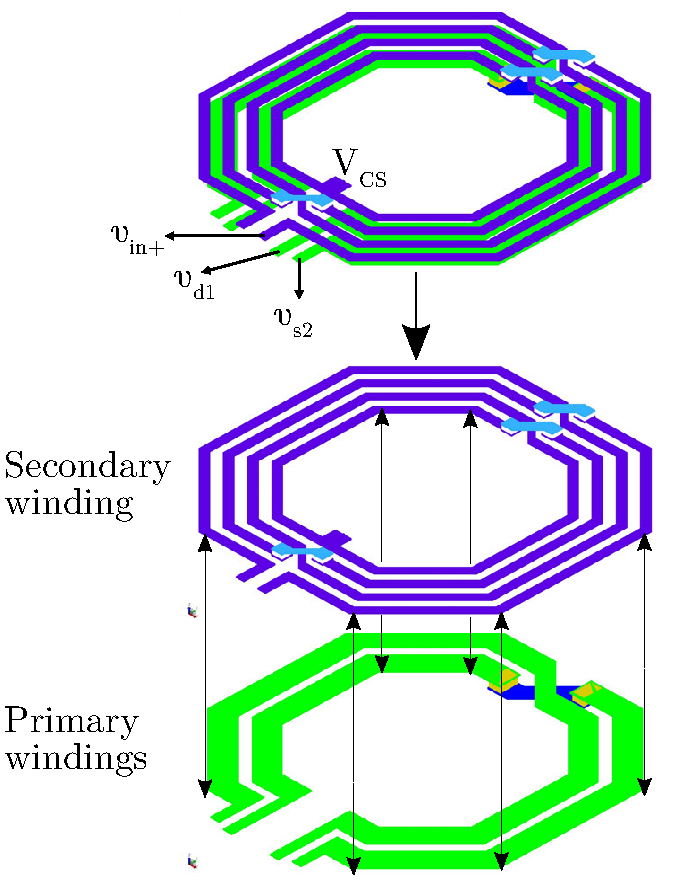
\includegraphics[width=0.6\linewidth]{assets/FD-SOI/Sub_6GHz_TRX_assets/LNA_inductors.pdf}
				\caption{Three-dimensional representation of the transformer used in the LNA of figure \ref{fig:FDSOI:TRX:LNA}. Figure taken from \cite{FDSOI2}.}
				\label{fig:FDSOI:LNA:transformers}
			\end{figure}

		Figure \ref{fig:FDSOI:TRX:IC} shows a photograph of the fabricated integrated circuit. The ratios of the LNA's input-transistors and the ratios of the output-transistors are $S_{1x}$ and $S_{2x}$, respectively.
		\begin{align*}
			&S_{1x}=\frac{W_{1x}}{L_{1x}}=\frac{0.9\unit{\milli\meter}}{28\unit{\nano\meter}}\approxeq 32,142.\overline{857\ 142}\\
			&S_{2x}=\frac{W_{2x}}{L_{2x}}=\frac{0.8\unit{\milli\meter}}{150\unit{\nano\meter}}\approxeq 5,333.\overline{3}
		\end{align*}
		\begin{figure}[h!]
			\centering
			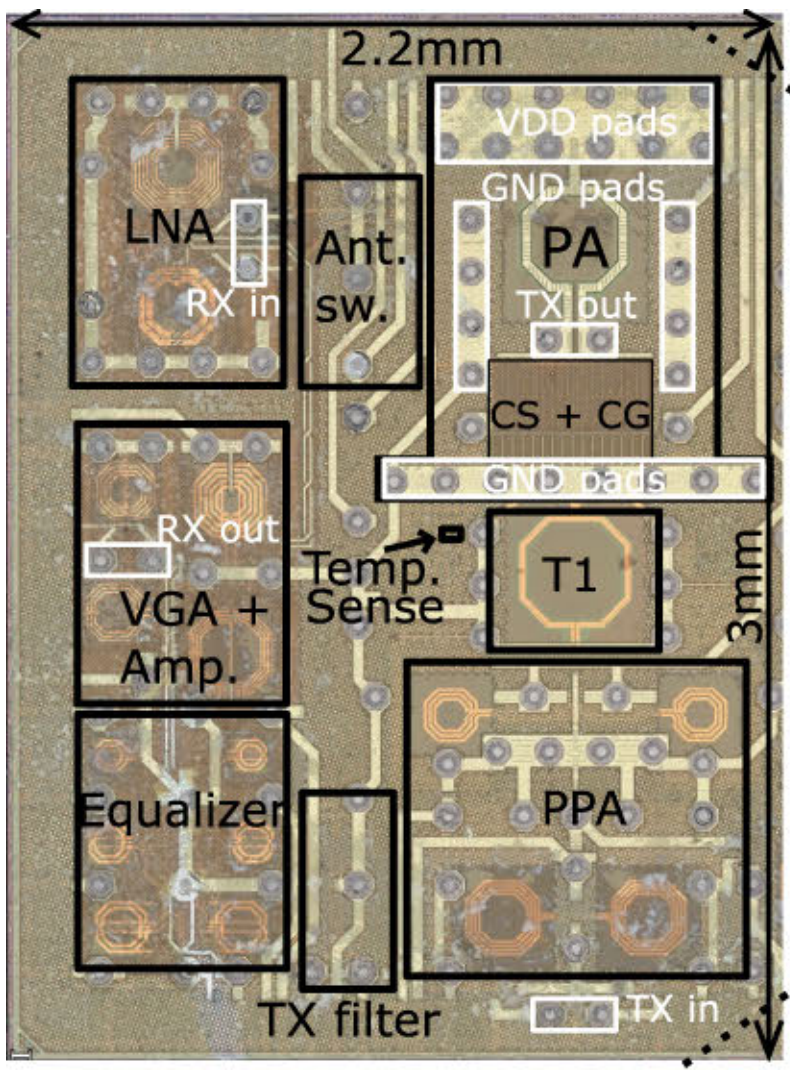
\includegraphics[width=0.7\linewidth]{assets/FD-SOI/Sub_6GHz_TRX_assets/IC.png}
			\caption{Photograph of the fabricated IC \cite{FDSOI2}.}
			\label{fig:FDSOI:TRX:IC}
		\end{figure}

		\begin{figure*}[ht!]
			\centering
			% \resizebox{1.5\linewidth}{!}{
\begin{tikzpicture}
    \node[shape=rectangle, fill={rgb,255:red,239;green,209;blue,209}, minimum width=6cm, minimum height=2.75cm] at (5, 3.125){};
    \node[shape=rectangle, fill={rgb,255:red,239;green,209;blue,209}, minimum width=6cm, minimum height=2.75cm] at (-5, 3.125){};
    \draw (-1, 5.25) to[cute inductor, l_=$L_g$] (-1, 6.25);
    \node[vcc, rotate=90](N1) at (-1.21, 5.75){} node[anchor=east] at ([xshift=0.12cm]N1.text){$V_{\symup{CS}}$};
    \node[circ, xscale=-1, yscale=-1] at (-1.21, 5.75){};
    \draw (1, 5.25) -- (1, 5);
    \node[circ] at (-1, 5){};
    \node[circ] at (1, 5){};
    \draw[-latex] (0.25, 5) -- (-0.25, 5);
    \draw (-1, 5) -- (-0.5, 5);
    \draw (0.5, 5) -- (1, 5);
    \node[ocirc] at (-0.5, 5){};
    \node[ocirc] at (0.5, 5){};
    \draw[-latex] (-0.667, 5) -- (-0.833, 5);
    \draw[-latex] (0.833, 5) -- (0.667, 5);
    \node[shape=rectangle, minimum width=0.465cm, minimum height=0.465cm](N2) at (-0.714, 4.75){} node[anchor=center] at (N2.text){$i_{\symup{in}}$};
    \node[shape=rectangle, minimum width=0.465cm, minimum height=0.436cm](N3) at (0.714, 4.765){} node[anchor=center] at (N3.text){$i_{\symup{in}}$};
    \draw[-latex] (-4.75, 5.25) -- (-4.75, 7.75);
    \node[shape=rectangle, minimum width=0.715cm, minimum height=0.715cm](N4) at (-4.375, 6.5){} node[anchor=center] at (N4.text){$v_{L_{dl}}$};
    \draw (-6, 6.5) to[cute inductor, l_={$L_{dl}$}] (-6, 5.25);
    \draw (-6, 7.75) to[american controlled voltage source, mirror, l_={$s\left( M_1 i_{L_g} - M_2 i_{dr}\right)$}] (-6, 6.75);
    \draw[dash pattern={on 1.6pt off 1.6pt}] (-6, 8) -- (-4.75, 8);
    \node[ocirc] at (-4.75, 8){};
    \draw[dash pattern={on 1.6pt off 1.6pt}] (-6, 5) -- (-4.75, 5);
    \node[ocirc] at (-4.75, 5){};
    \node[circ] at (-6, 8){};
    \node[circ] at (-6, 5){};
    \draw[-latex] (4.75, 5.25) -- (4.75, 7.75);
    \node[shape=rectangle, minimum width=0.715cm, minimum height=0.715cm](N5) at (4.375, 6.5){} node[anchor=center] at (N5.text){$v_{L_{dr}}$};
    \draw[dash pattern={on 1.6pt off 1.6pt}] (4.75, 5) -- (6, 5);
    \draw[dash pattern={on 1.6pt off 1.6pt}] (4.75, 8) -- (6, 8);
    \node[ocirc] at (4.75, 5){};
    \node[shape=rectangle, minimum width=0.715cm, minimum height=0.715cm](N6) at (5.625, 8.5){} node[anchor=center] at (N6.text){$i_{dr}$};
    \draw (6, 6.5) to[cute inductor, mirror, l={$L_{dr}$}] (6, 5.25);
    \node[circ] at (6, 8){};
    \node[circ] at (6, 5){};
    \draw (1, 6.25) to[american controlled voltage source, l={$s M_1 \left(i_{dl} - i_{dr}\right)$}] (1, 5.25);
    \draw (-6, 9) -- (-6, 7.75);
    \draw (-6, 5.25) -- (-6, 4);
    \draw (-6, 6.75) -- (-6, 6.5);
    \node[ocirc] at (-6, 9){};
    \draw[-latex] (-6, 8.75) -- (-6, 8.25);
    \node[shape=rectangle, minimum width=0.715cm, minimum height=0.715cm](N7) at (-5.625, 8.5){} node[anchor=center] at (N7.text){$i_{dl}$};
    \draw (6, 5.25) -- (6, 4);
    \draw (6, 7.75) to[american controlled voltage source, mirror, l={$s\left( -M_1 i_{L_g} - M_2 i_{dl}\right)$}] (6, 6.75);
    \draw (6, 9) -| (6, 7.75);
    \draw[-latex] (6, 8.75) -- (6, 8.25);
    \node[ocirc] at (6, 9){};
    \node[ocirc] at (4.75, 8){};
    \draw (6, 6.75) -| (6, 6.5);
    \draw (-6, 4) to[american controlled current source, l_={$g_m^{\text{\tiny{(11)}}} v_{gs}^{\text{\tiny{(11)}}}$}] (-6, 3);
    \draw (-3.5, 4) to[capacitor, l_={$C_{gs}^{\text{\tiny{(11)}}}$}] (-3.5, 3);
    \draw (-6, 3) -| (-6, 2.5) -| (-3.5, 3);
    \node[shape=rectangle, minimum width=0.715cm, minimum height=0.715cm](N8) at (-2.625, 3.5){} node[anchor=center] at (N8.text){$v_{gs}^{\text{\tiny{(11)}}}$};
    \draw[-latex] (-3, 3) -- (-3, 4);
    \draw (-3.5, 4) -| (-3.5, 5) -- (-1, 5);
    \draw (6, 4) to[american controlled current source, l={$g_m^{\text{\tiny{(12)}}} v_{gs}^{\text{\tiny{(12)}}}$}] (6, 3);
    \draw (3.5, 4) to[capacitor, l={$C_{gs}^{\text{\tiny{(12)}}}$}] (3.5, 3);
    \node[shape=rectangle, minimum width=0.715cm, minimum height=0.715cm](N9) at (2.625, 3.5){} node[anchor=center] at (N9.text){$v_{gs}^{\text{\tiny{(12)}}}$};
    \draw[-latex] (3, 3) -- (3, 4);
    \draw (3.5, 3) -| (3.5, 2.5) -| (6, 3);
    \draw (1, 5) -- (3.5, 5) -- (3.5, 4);
    \draw (-1, 5.25) -| (-1, 5);
    \draw (-1, 6.25) -| (-1, 6.5) -| (1, 6.25);
    \node[shape=rectangle, minimum width=0.715cm, minimum height=0.465cm](N10) at (0, 4.75){} node[anchor=center] at (N10.text){$v_{\symup{in}}$};
    \draw (-4.75, 2.5) -| (-4.75, 2) -| (4.75, 2.5);
    \node[circ] at (-4.75, 2.5){};
    \node[circ] at (0, 2){};
    \node[circ] at (4.75, 2.5){};
    \draw (0, 2) to[cute inductor, l={$L_{\symup{deg}}$}] (0, 0.5);
    \node[tlground] at (0, 0.5){};
    \node[shape=rectangle, minimum width=0.465cm, minimum height=0.465cm](N11) at (-3.75, 4.25){} node[anchor=center] at (N11.text){$\symup{G}$};
    \node[shape=rectangle, minimum width=0.465cm, minimum height=0.465cm](N12) at (3.75, 4.25){} node[anchor=center] at (N12.text){$\symup{G}$};
    \node[shape=rectangle, minimum width=0.465cm, minimum height=0.465cm](N13) at (-5.75, 4.25){} node[anchor=center] at (N13.text){$\symup{D}$};
    \node[shape=rectangle, minimum width=0.465cm, minimum height=0.465cm](N14) at (5.75, 4.25){} node[anchor=center] at (N14.text){$\symup{D}$};
    \node[shape=rectangle, minimum width=0.465cm, minimum height=0.465cm](N15) at (5, 2.25){} node[anchor=center] at (N15.text){$\symup{S}$};
    \node[shape=rectangle, minimum width=0.465cm, minimum height=0.465cm](N16) at (-5, 2.25){} node[anchor=center] at (N16.text){$\symup{S}$};
    \node[shape=rectangle, minimum width=0.465cm, minimum height=0.465cm](N17) at (0, 6.75){} node[anchor=center] at (N17.text){$i_{L_{g}}$};
    \draw[-latex] (0.25, 6.5) -- (-0.25, 6.5);
\end{tikzpicture}
% }
			\caption{Small signal equivalent of figure \ref{fig:FDSOI:TRX:LNA} with reactive series-shunt feedback. Transistors $\symup{M_{21}}$ and $\symup{M_{22}}$ are omitted from the model for clarity.}
			\label{fig:FDSOI:TRX:LNA_REACTIVE_FEEDBACK}
		\end{figure*}

	\ifCLASSOPTIONcaptionsoff
		\newpage
	\fi

	\printbibliography
\end{document}